
\begingroup
\let\clearpage\relax
\chapter{问题与背景}

\section{研究背景}

人类能够很简单的从几个有限的样例中提取事物的特征并且进行区分,但是这对于现代机器学习来说还是很大的挑战。
经典的元学习模型用来解决小样本学习问题,包括两个部分,分别是将输入域映射到特征空间的嵌入模型,和将特征空间映射到目标变量的基本学习器。

虽然目前有很多可以选择的基础学习器,但最临近分类器以及其变体是最常用的(例如\upcite{snell2017prototypical,vinyals2016matching})。
然而线性分类器能很好的利用更加丰富的反面数据,更好的学习类别的边界,从而使其表现优于最邻近分类器。

本文研究了以线性分类器作为基础学习器的元学习问题。
% 本文使用线性支持向量机构建一个分类器,
由于元学习的目标是让模型具有良好泛化性,因此需要在不同任务之间最小化泛化误差,这通常需要使用循环优化的方法
来训练线性分类器,带来了很大的计算量。因此可计算性是此问题的关键。

然而,线性模型的目标函数是通常是凸的,因此这个问题可以被有效解决。
在小样本的环境下,凸优化可以使元学习变得高效。
本文观察到凸的性质中引出的两个额外特性,优化的隐式可微性和分类器的低秩特性\upcite{barratt2018differentiability,gould2016differentiating}。
第一个特性允许使用一个已有的凸优化模型估计最优值,并隐式地微分最优性条件或卡罗需-库恩-塔克(Karush-Kuhn-Tucker,KKT)条件来训练嵌入模型。
第二个特性是对于小样本学习,对偶形式中的待优化变量数目远小于特征维数,通过构造对偶优化问题可以大大减少优化变量的个数。

% 利用以上两个特性,本文实现了在计算成本略有增加的情况下提供了比最临近分类器更大的收益。

\section{国内外研究}
元学习探究学习器在不同任务上的泛化能力的影响因素\upcite{schmidhuber1987evolutionary,thrun1998lifelong,vilalta2002perspective}。
用于少样本学习的元学习方法可以大致分为三组
一是基于梯度的方法\upcite{ravi2017optimization,finn2017model},它通过梯度下降方法寻找和修改嵌入模型的参数。
二是最近邻方法\upcite{vinyals2016matching,snell2017prototypical},它在样本的嵌入特征上学习基于距离的预测规则。
三是基于模型的方法\upcite{mishra2017simple,munkhdalai2018rapid},学习一个参数化的预测器来估计模型参数。

本文的工作主要与用后向传播进行过程优化的技术相关。
Domke\upcite{domke2012generic} 提出了一种基于固定步数的梯度下降和自动微分计算梯度的通用方法。
但是由于需要计算梯度,优化器的优化过程中间值需要被记录,这会需要很大的存储空间,应用于规模较大
的问题是不现实的。
然而,优化器的轨迹(中间值)需要存储以计算梯度,这可能会对大问题造成限制。
Maclaurin 等人考虑了存储开销问题\upcite{maclaurin2015gradient},他们研究了深度网络优化轨迹的低精度表示。
如果可以在分析上找到优化的最小值,例如无约束的二次最小化问题,分析的计算梯度也可以被接受。
这个成果已经应用于低层视觉问题中\upcite{tappen2007learning,schmidt2014shrinkage}。

本文的方法使用线性分类器,因为它能够规划为凸学习问题。
特别是对于目标函数是一个二次规划问题(QP),可以基于梯度技术高效的获得全局最优解。
此外,凸问题的解可以由它们的KKT条件所描述,
这使得我们可以使用隐函数定理通过学习者\upcite{krantz2002implicit}进行反向传播。
具体而言,本文使用了Amos和Kolter的公式化方法\upcite{amos2017optnet},
该方法提供了计算QP及其梯度的高效GPU程序。虽然他们将这个框架应用于学习约束满足问题的表示,
但由于出现的问题规模通常很小,因此它也非常适合少样本学习。\\

\vspace*{6pt}

\endgroup

\begingroup
\let\clearpage\relax
\chapter{解决方案}
\section{问题描述}
给定训练集 $D^{train} = \{(x_t,y_t)\}^{T}_{t=1}$ ,基学习器 $A$ 的目标是利用参数 $\theta$ 对预测器 $y=f(x,\theta)$ 进行估计,
以在未见的测试集 $D^{test} = \{(x_a, y_a)\}^{Q}_{t=1}$ 上实现更好的泛化能力,
% 通常假设训练集和测试集采样自相同分布,并使用参数 $\phi$的嵌入模型$f_{\phi}$将样本域映射到特征空间。
% 对于基于优化的学习器,参数通过最小化训练数据上的经验损失以及正则项获得。
\begin{equation}
    \label{equation:1}
    \theta = A(D^{train}; \phi) = \mathrm{arg\,min}_{\theta}L^{base}(D^{train}; \theta, \phi) + R(\theta)
\end{equation}
其中,$L^{base}$ 是损失函数,$R(\theta)$ 是正则项,在训练数据有限的情况下,正则项在模型的泛化方面扮演很重要的角色。

为了最小化泛化误差,少样本元学习方法旨在学习任务分布中的最优模型,这可以看作是在一个任务集合上进行学习:
$T = \{(D_{i}^{train}, D_{i}^{test})\}^{I}_{i=1}$,通常被称为元训练集。
% 通过元组$(D_i^{train}, D_i^{test})$描述的训练和测试数据集。
本文的目标是学习一个嵌入模型$\phi$,使得在给定基础学习者$A$的情况下,在不同任务中达到最小化泛化(或测试)误差的效果。

为了实现这一目标,本文的学习目标是:
\begin{equation}
    \label{equation:2}
    \min_{\phi} \mathbb{E}_{T} [L^{meta}(D^{test}; \theta, \phi), \mathrm{where} \, \theta = A(D^{train}, \phi)]
\end{equation}

\begin{figure}[htbp]
    \centering
    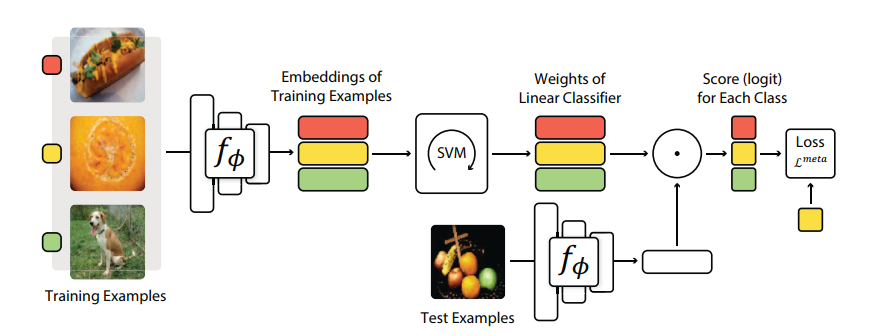
\includegraphics[width=.7\linewidth]{figure/p1.png}
    \caption{Overview of our approach.}
    \label{fig:1}
\end{figure}

图\ref{fig:1} 展示了单一任务的训练和测试过程。一旦学习到嵌入模型 $f_{\phi}$,它的泛化性能可以在一个保留的任务集合(通常称为元测试集)上进行评估。元测试集 
$S = \{(D_j^{train}, D_j^{test})\}^J_{j=1}$ 可以用公式来计算:
\begin{equation}
    \label{equation:3}
    \mathbb{E}_S[L^{meta}(D^{test}; \theta, \phi), \mathrm{where} \, \theta = A(D^{train}; \phi)]
\end{equation}

根据之前的研究\upcite{ravi2017optimization,finn2017model},公式 \ref{equation:2} 和 公式\ref{equation:3}
中期望值的估计分别被称为元训练和元测试阶段。
% 在元训练阶段,本文会保留一个额外的验证集来选择元学习器的超参数并挑选最佳的嵌入模型。

% \section{创新思想}
% 本文将可微的二次规划求解器和不同的线性分类器综合起来。利用以上两个特性,本文实现了在
% 计算成本略有增加的情况下提供了比最临近分类器更大的收益。

% 本文利用线性分类器的凸优化性质,将线性分类器作为基础学习器应用于元学习,用于解决可计算性问题。


\section{具体方法}
\subsection{任务集}
少样本学习使用K-way,N-shot分类任务对模型进行评估,
其中K表示类别数,$N$表示每个类别的训练样本数,
% 如$N\in{1,5}$。
% 虽然 miniImageNet\upcite{ravi2017optimization} 等数据集没有明确给出训练集和测试集$(D_i^{train}, D_i^{test})$,
这被称为任务集。
一个任务集 $\tau_i=(D_i^{train}, D_i^{test})$ 可以按以下方式进行采样\upcite{ravi2017optimization,vinyals2016matching}:

总体类集为$C^{train}$, 对于每个任务集,首先类$C_i$(包含来自$C^{train}$的K类)被有放回抽样得到,
训练集$D_i^{train} = \{(x_n, y_n) | n=1,...,N \times K, y_n \in C_i\}$(每个类包含N个图像)被采样,
测试集$D_i^{test} = \{(x_n, y_n) | n = 1,...,Q \times K, y_n \in C_i\}$(每个类包含Q个图像)被采样。

需要满足$D_i^{train} \cap D_i^{test} = \emptyset $,以优化泛化误差。以同样的方式从$C^{val}$
和$C^{test}$各自构造元验证集(meta-validation)和元测试集(meta-test)。
为了度量嵌入模型对未见类的泛化,$C^{train}, C^{val}, C^{test}$需被互斥选择。

\subsection{凸基学习器}

% 当选择基学习器$A$时,必须考虑计算的效率,因为基学习器的计算效率直接影响到公式\ref{equation:2}中期望值的计算。
% 同时,在估计嵌入模型参数$\phi$时,也必须能够有效地计算任务测试误差$L^{meta}(D^{test}; \theta,\phi)$相对于$\phi$的梯度,
% 这促使简单的基学习器出现,例如最近类别平均值\upcite{snell2017prototypical},其中基学习器$\theta$的参数易于计算,且目标是可微的。

本文考虑基于多类线性分类器的基学习器(例如支持向量机(SVM)、逻辑回归和岭回归)\upcite{crammer2001algorithmic,weston1999support},
其中基学习器的目标是凸的。例如,K类线性SVM可以写成$\theta = \{w_k\}^K_{k=1}$的形式。Crammer和Singer\upcite{crammer2001algorithmic}提出的多类支持向量机的公式是:
\begin{equation}
    \label{equation:4}
\begin{aligned}
   & \theta = A(D^{train}; \phi) = \arg \min_{\{w_k\}}\min_{\{\xi_k\}}\frac{1}{2}\Sigma_k||w_k||_2^2 + C \Sigma_n \xi_n\\
   & \mathrm{subject \, to} \\
   & w_{y_n} \cdot f_{\phi}(x_n)-w_k \cdot f_\phi (x_n) \ge 1 - \delta_{y_n,k} - \xi_n, \forall n, k\\
\end{aligned}
\end{equation}
这个公式中的 $D^{train} = \{(x_n, y_n)\}$ 表示训练集,其中每个样本 $x_n$ 都有一个真实标签 $y_n$。
$C$ 是一个正则化参数,用于控制模型的复杂度和泛化能力。$δ_{·,·}$是克罗内克(Kronecker)$δ$ 函数.

\subsubsection{SVM目标函数的梯度}

从图\ref{fig:1} 中可以看出,为了实现端到端的训练,本文需要对SVM求解器的解进行微分,以便计算出
$\{\frac{\partial\theta}{\partial f_\phi(x_n)}\}^{N \times K}_{n=1}$。
由于SVM的目标是凸优化问题,因此具有唯一的最优解,可以在最优(KKT)条件下使用隐函数定理来获得所需的梯度。
本文还推导了该凸优化问题的隐函数定理形式\upcite{bertinetto2018meta},考虑以下凸优化问题:
\begin{equation}
    \label{equation:5}
    \begin{aligned}
        \mathrm{minimize} \; &f_0(\theta, z)\\
        \mathrm{subject\, to} &f(\theta, z) \le 0\\
        &h(\theta, z)=0\\
    \end{aligned}
\end{equation}
其中向量$\theta \in \mathbb{R}^d$是问题的优化变量,向量$z \in \mathbb{R}^e$是优化问题的输入参数,即在本文的情况下是$\{f_\phi(x_n)\}$。
本文可以通过求解以下拉格朗日函数的鞍点$(\tilde{\theta}, \tilde{\lambda}, \tilde{\nu})$来优化目标:
\begin{equation}
    \label{equation:6}
    L(\theta, \lambda, \nu, z) = f_0(\theta, z) + \lambda^{T} f(\theta, z) + \nu^Th(\theta, z)
\end{equation}
换言之,本文可以通过解决 $g(\tilde{\theta}, \tilde{\lambda}, \tilde{\nu}, z  ) = 0$ 来获得目标函数的最优解,其中
\begin{equation}
    \label{equation:7}
    g(\theta, \lambda, \nu, z ) = \left [
        \begin{array}{l}
            \nabla_\theta L(\theta, \lambda, \nu,z)\\
            \mathbf{diag}(\lambda)f(\theta, z)\\
            h(\theta, z)
        \end{array}
        \right ]
\end{equation}
对于一个函数 $f(x) : \mathbb{R}^n \rightarrow \mathbb{R}^m$,将$D_xf(x)$ 表示为它的 Jacobian 矩阵 $\in \mathbb{R}_{m\times n}$.

\subsubsection{定理1}
(来自Barratt\upcite{barratt2018differentiability})假设 $g(\tilde{\theta}, \tilde{\lambda}, \tilde{\nu}, z  ) = 0$ 。当所有导数都存在时,
\begin{equation}
    \label{equation:8}
    D_z\tilde{\theta} = -D_{\theta}g(\tilde{\theta}, \tilde{\lambda}, \tilde{\nu}, z)^{-1}D_zg(\tilde{\theta}, \tilde{\lambda}, \tilde{\nu}, z)
\end{equation}
通过应用隐函数定理于KKT条件,本文得到了最优解$\tilde{\theta}$对输入数据梯度的闭合形式表达式,这是凸问题相对于通用优化问题的优势之一。
由此,本文不需要反向传播整个优化轨迹来计算梯度,也不需要消耗过多的内存。由于最优解的唯一性,这种方法是可行的。

% \subsubsection{时间复杂度}
% 为了在前向传递过程中应用该方法(公式\ref{equation:4}),需要进行QP求解,其时间复杂度为$O(d^3)$,其中$d$是优化变量的数量。
% 主要的时间消耗在分解KKT矩阵上,这是原始对偶内点法的基本操作。
% 在后向传递过程中,需要使用定理1来解决公式\ref{equation:8},其复杂度为$O(d^2)$(前提是在前向传递过程中已进行矩阵分解)。
% 当嵌入维度较大时,前向和后向传递的成本都很高。

\subsubsection{对偶学习}

由于公式\ref{equation:4}中的目标对偶规划本身具有处理嵌入维度上的低依赖性,因此可以重写为如下形式:
令
\begin{equation}
    \label{equation:9}
    w_{k}(\alpha^{k}) = \sum_{n}{\alpha_{n}^{k} f_{\phi}(x_{n})} \quad \forall k.
\end{equation}
可以在对偶空间优化  
\begin{equation}
    \label{equation:10}
    \begin{aligned}
        &\mathrm{max}_{\alpha ^{k}} \big[ -\frac{1}{2} \sum_{k}\parallel\omega_{k}(\alpha^{k})\parallel_{2}^{2} + \sum_{n}\alpha_{n}^{y_{n}}\big]\\ 
        &\mathrm{subject \, to} \quad \alpha_{n}^{y_{n}} \leq C, \ \alpha_{n}^{k} \leq 0 \quad \forall k \neq y_{n} , \\ 
        &\qquad \sum_{k}{\alpha_{n}^{k}=0 \quad \forall n.}\\
    \end{aligned}
\end{equation}
本文可以将公式\ref{equation:4}重写为一个在对偶变量$\{\alpha^k\}^K_{K=1}$上的二次规划(QP),
% 这里的优化变量数量是训练样本数量乘以类数,通常比特征维度的数量小,特别适用于少样本学习。
为了解决对偶二次规划,本文使用了一个可微的基于GPU的QP求解器\upcite{amos2017optnet}。
% 实践表明,QP求解所需的时间与使用ResNet-12计算特征的时间相当,因此与使用基于简单基学习器(例如Prototypical Networks中使用的最近类原型均值)相比,
% 每次迭代的总体速度没有太大差异\upcite{snell2017prototypical}。

同时,Bertinetto \upcite{bertinetto2018meta} 也采用了岭回归作为基学习器,
% 并且它也有一个闭式解。尽管岭回归可能不是最适合分类问题的模型,但是它的工作表明,在实践中,
% 通过最小化关于one-hot标签的平方误差来训练模型可以起到很好的效果。最终,
对于岭回归,优化问题也是一个QP,因此可以在本文的框架中实现:
\begin{equation}
    \label{equation:11}
    \mathrm{max}_{\alpha^{k}} \big[ - \frac{1}{2} \sum_{k} \parallel\omega_{k}(\alpha^{k}) \parallel_{2}^{2} - \frac{\lambda}{2} \sum_{k}{\parallel\alpha^{k}\parallel_{2}^{2}}+\sum_{n}{\alpha_{n}^{y_{n}}} \big] 
\end{equation}
其中$w_k$定义同公式\ref{equation:9}。

% 线性SVM和岭回归之间的比较表明线性SVM规划具有稍微优势。

\subsection{元学习目标}

为了评估模型的性能,
% 本文评估从同一任务中采样的测试数据的负对数似然。因此,
本文可以将公式\ref{equation:2}的元学习目标重新表达为:
\begin{equation}
    \label{equation:12}
    L^{meta}(D^{test};\theta,\phi,\gamma)=\sum_{(x,y) \in D^{test}}{ \big[ -\gamma \omega_{y} \cdot f_{\phi}(x) + \mathrm{log}\sum_{k}{\mathrm{exp}(\gamma\omega_{k}\cdot f_{\phi}(x))}\big]}
\end{equation}
其中$\theta=A(D^{train};\phi)=\{\omega_{k}\}_{k=1}^{K}$,$\gamma$是一个可学习的缩放参数。\\

\vspace*{6pt}
% 之前的研究表明\upcite{oreshkin2018tadam,bertinetto2018meta,gidaris2018dynamic},通过可学习的比例因子$\gamma$调整预测分数,在最近类别均值和岭回归基学习器下可以提高性能
   
\endgroup
\begingroup
\let\clearpage\relax

\chapter{实验与分析}

% \section{创新思想和学术贡献}

% 在本文中,本文提出了一种基于凸基学习器的元学习方法用于少样本学习。
% 对偶形式和KKT条件可用于实现计算和存储效率高的元学习,因此特别适用于少样本学习问题。
% 与最近邻分类器相比,线性分类器在稍微增加计算成本的情况下提供更好的泛化能力。
% 本文的实验表明,正则化的线性模型允许更高的嵌入维度,并减少了过度拟合。对于未来的工作,
% 本文旨在探索其他凸基学习器,如核SVM。这将允许随着更多的训练数据可用于任务而逐渐增加模型容量的能力。

% \section{实验方法}
% 首先,本文描述了在实验中使用的网络架构和优化细节。
% 然后,本文展示了在标准的几种少样本分类基准上的结果,包括ImageNet的派生数据集和CIFAR,
% 随后本文使用相同的嵌入网络和训练设置对各种基础学习器对准确性和速度的影响进行了详细分析。
\section{实验设置}
在元学习设置方面,本文在实验中使用了一个ResNet-12网络,遵循\upcite{oreshkin2018tadam,mishra2017simple}。
% 令Rk表示由三个{3×3卷积和k个滤波器,批归一化,Leaky ReLU(0.1)}组成的残差块;令MP表示2×2最大池化。
% 本文使用了DropBlock正则化\upcite{ghiasi2018dropblock},
% 一种结构化Dropout形式。令DB(k,b)表示具有保持率为k和块大小为b的DropBlock层。
用于ImageNet衍生数据集的网络架构为:R64-MP-DB(0.9,1)-R160-MP-DB(0.9,1)-R320-MP-DB(0.9,5)-R640-MP-DB(0.9,5),
而用于CIFAR衍生数据集的网络架构为:R64-MP-DB(0.9,1)-R160-MP-DB(0.9,1)-R320-MP-DB(0.9,2)-R640-MP-DB(0.9,2)。
本文使用带有0.9的Nesterov动量和0.0005的权重衰减的SGD作为优化器。
% 该模型进行了60个epochs的元训练,每个epoch包含1000个样本集。
学习率最初设置为0.1,然后在第20、40和50个epoch时分别更改为0.006、0.0012和0.00024,这是遵循\upcite{gidaris2018dynamic}的实践。

在元训练期间,本文采用了水平翻转、随机裁剪和颜色(亮度、对比度和饱和度)扰动数据增强,如\upcite{gidaris2018dynamic,qiao2018few}中所述。
本文在两个阶段都使用5路分类,这是遵循最近的工作\upcite{gidaris2018dynamic,oreshkin2018tadam}。
对于原型网络,本文将元训练shot设置为与元测试shot相匹配,这是遵循\upcite{snell2017prototypical,gidaris2018dynamic}的做法。
对于SVM和岭回归,本文观察到保持元训练shot高于元测试shot可以获得更好的测试准确性,如 图\ref{fig:2} 所示。因此,在元训练期间,
本文针对ResNet-12的miniImageNet将训练shot设置为15;对于使用4层CNN的miniImageNet(在表\ref{table:3}中)将训练shot设置为5;
对于tieredImageNet,将训练shot设置为10;对于CIFAR-FS,将训练shot设置为5;对于FC100,将训练shot设置为15。

\begin{figure}[htbp]
    \centering
    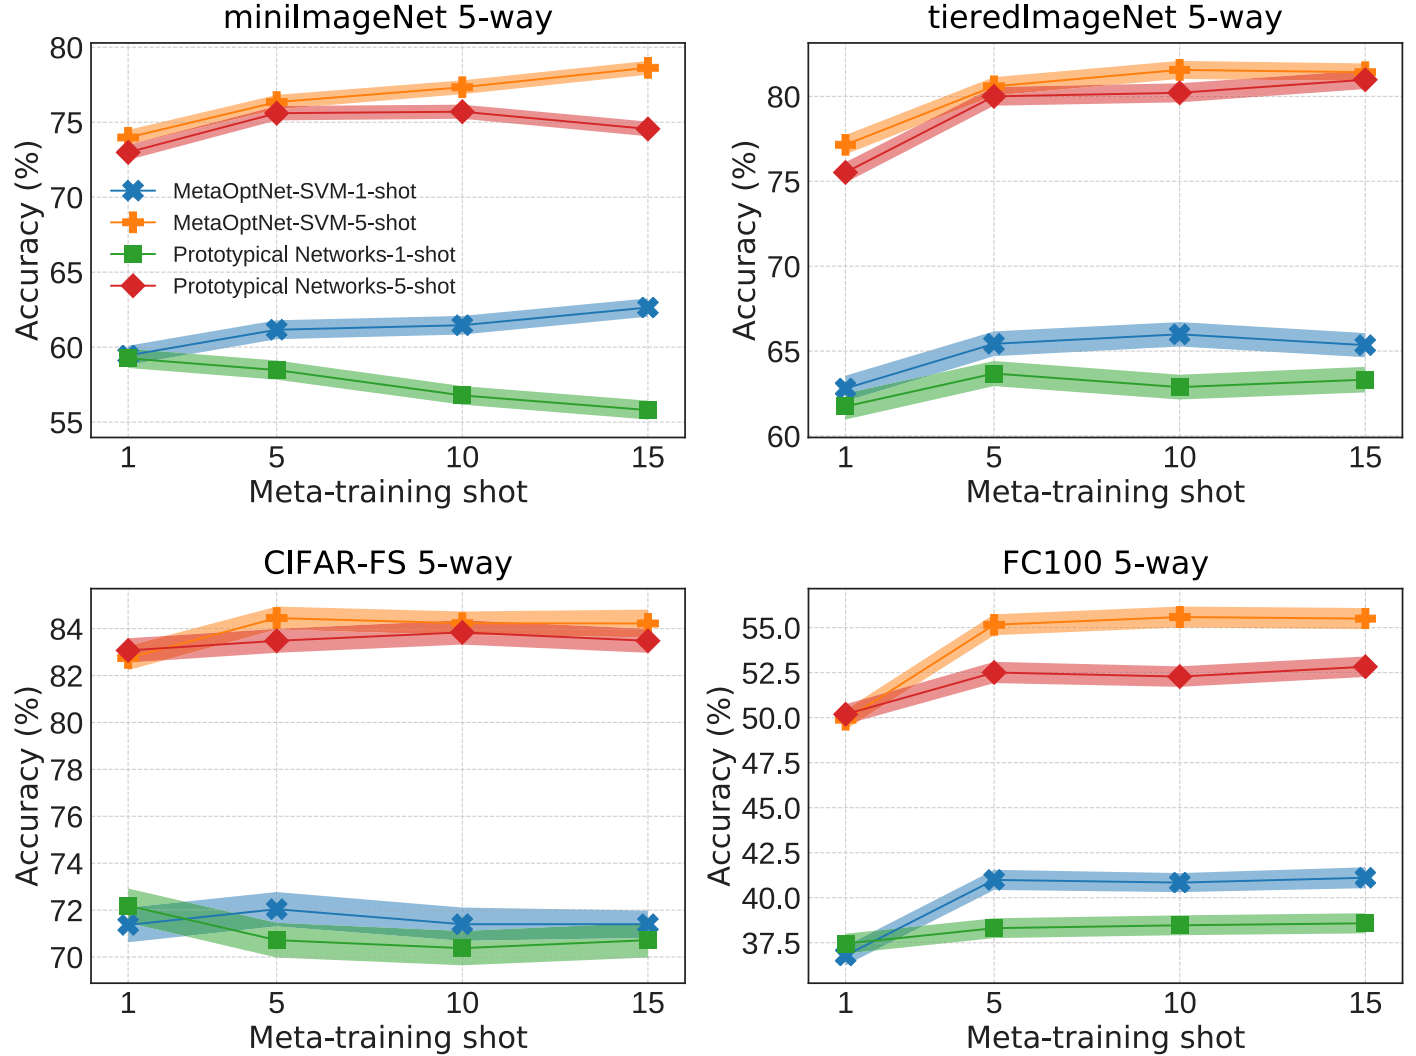
\includegraphics[width=.6\linewidth]{figure/f2.png}
    \caption{使用不同的元训练样本数量,在miniImageNet元测试集上的测试准确率(\%)。}
    \label{fig:2}
\end{figure}

% 在基学习器的设置方面,对于线性分类器的训练,本文使用二次规划求解器OptNet \upcite{amos2017optnet}。
% SVM的正则化参数C设置为0.1。岭回归的正则化参数λ设置为50.0。对于最近类均值(原型网络),
% 本文使用针对特征维度进行归一化的平方欧氏距离。

% 在提前停止方面,虽然本文可以运行优化器直到收敛,但在实践中,本文发现在固定的迭代次数(仅三次)
% 内运行QP求解器实际上效果很好。提前停止起到了额外的正则化作用,甚至可以带来稍微更好的性能。


\subsection{在ImageNet的衍生数据集上的实验}

miniImageNet数据集\upcite{vinyals2016matching}是用于少样本图像分类的标准基准测试,
由ILSVRC-2012 \upcite{russakovsky2015imagenet}中随机选择的100个类组成。
tieredImageNet基准测试\upcite{ren2018meta}是ILSVRC-2012 \upcite{russakovsky2015imagenet}的一个较大子集,由608个类别组成,分为34个高级类别。
表\ref{table:1}总结了5-way miniImageNet和tieredImageNet上的结果。在miniImageNet和tieredImageNet元测试集上,
使用95\%置信区间的平均few-shot分类准确率(\%)。“a-b-c-d”表示每个层中具有a,b,c和d个滤波器的4层卷积网络。
†表示使用元训练集和元验证集的并集来元训练元学习器。“RR”代表岭回归。
\begin{table}[htbp]
    \caption{与之前在miniImageNet和tieredImageNet上的工作进行比较}
    \resizebox{\linewidth}{!}{  
    \begin{tabular}{
    l 
    l 
    c 
    c 
    l 
    l }
    \toprule 
                                                     &                                   & \multicolumn{2}{c}{\textbf{miniImageNet 5-way}}                                                               & \multicolumn{2}{c}{\textbf{tieredImageNet 5-way}}                                                 \\ \cline{3-6} 
    \textbf{model}                                   & \textbf{backbone}                 & \textbf{1-shot}                                                   & \textbf{5-shot}                                                   & \multicolumn{1}{c}{\textbf{1-shot}} & \multicolumn{1}{c}{\textbf{5-shot}} \\ \hline
    Meta-Learning LSTM*                              & 64-64-64-64                       & 43.44 ± 0.77                                                      & 60.60 ± 0.71                                                      & -                                                           & -                                                           \\
    Matching Networks*                               & 64-64-64-64                       & 43.56 ± 0.84                                                      & 55.31 ± 0.73                                                      & -                                   & -                                   \\
    MAML                                             & 32-32-32-32                       & 48.70 ± 1.84                                                      & 63.11 ± 0.92                                                      & 51.67 ± 1.81                                                & 70.30 ± 1.75                                                \\
    Prototypical Networks*                           & 64-64-64-64                       & 49.42 ± 0.78                                                      & 68.20 ± 0.66                                                      & 53.31 ± 0.89                                                & 72.69 ± 0.74                                                \\
    Relation Networks*                               & 64-96-128-256                     & 50.44 ± 0.82                                                      & 65.32 ± 0.70                                                      & 54.48 ± 0.93                                                & 71.32 ± 0.78                                                \\
    R2D2                                             & 96-192-384-512                    & 51.2 ± 0.6                                                        & 68.8 ± 0.1                                                        & -                                   & -                                   \\
    Transductive Prop Nets                           & 64-64-64-64                       & 55.51 ± 0.86                                                      & 69.86 ± 0.65                                                      & 59.91 ± 0.94                                                & 73.30 ± 0.75                                                \\
    SNAIL                                            & ResNet-12                         & 55.71 ± 0.99                                                      & 68.88 ± 0.92                                                      & -                                   & -                                   \\
    Dynamic Few-shot                                 & 64-64-128-128                     & 56.20 ± 0.86                                                      & 73.00 ± 0.64                                                      & -                                   & -                                   \\
    AdaResNet                                        & ResNet-12                         & 56.88 ± 0.62                                                      & 71.94 ± 0.57                                                      & -                                   & -                                   \\
    TADAM                                            & ResNet-12                         & 58.50 ± 0.30                                                      & 76.70 ± 0.30                                                      & -             -                                   \\
    Activation to Parameter† & WRN-28-10                         & 59.60 ± 0.41                                                      & 73.74 ± 0.19                                                      & -                                   & -                                   \\
    LEO                                              & WRN-28-10                         & 61.76 ± 0.08                                                      & 77.59 ± 0.12                                                      & 66.33 ± 0.05                                                & 81.44 ± 0.09                                                \\
    MetaOptNet-RR (ours)                             & ResNet-12 & 61.41 ± 0.61                                                      & 77.88 ± 0.46                                                      & \textbf{65.36 ± 0.71}                                       & \textbf{81.34 ± 0.52}                                       \\
    MetaOptNet-SVM (ours)                            & ResNet-12                         & 62.64 ± 0.61                                                      & 78.63 ± 0.46                                                      & \textbf{65.99 ± 0.72}                                       & \textbf{81.56 ± 0.53}                                       \\
    MetaOptNet-SVM-trainval (ours)†                  & ResNet-12                         & \textbf{64.09 ± 0.62} & \textbf{80.00 ± 0.45} & \textbf{65.81 ± 0.74}                                       & \textbf{81.75 ± 0.53}                                       \\
    \bottomrule
    \end{tabular}
    }
    \label{table:1}
\end{table}
本文的方法在5-way miniImageNet和tieredImageNet基准测试上取得了最先进的性能。
% 需要注意的是,LEO \upcite{rusu2018meta}除了使用WRN-28-10主干网络外,还利用编码器和关系网络来产生梯度下降的样本相关初始化。
% TADAM \upcite{oreshkin2018tadam}为每个卷积层使用任务嵌入网络(TEN)块,用于预测元素级比例和偏移向量。

% 本文还注意到,\upcite{rusu2018meta,qiao2018few}对WRN-28-10特征提取器\upcite{zagoruyko2016wide}进行了预训练,以共同分类miniImageNet元训练集中的全部64个类别;然后在元训练期间冻结网络。
% \upcite{oreshkin2018tadam}使用了一种类似的策略,使用标准分类任务:他们同时在few-shot分类任务(5-way)和标准分类任务(64-way)上联合训练特征嵌入。
% 相比之下,
% 本文的系统是端到端进行元训练的,明确地训练特征提取器在带有正则化线性分类器的few-shot学习任务上表现良好。

\subsection{CIFAR派生数据集的实验}

CIFAR-FS数据集\upcite{bertinetto2018meta}是最近提出的few-shot图像分类基准测试,
由CIFAR-100 \upcite{krizhevsky2010cifar}中的全部100个类别组成。
FC100数据集\upcite{oreshkin2018tadam}是另一个源自CIFAR-100 \upcite{krizhevsky2010cifar}的数据集,包含100个类别,这些类别被分成20个超类。
表\ref{table:2}总结了5-way分类任务的结果,本文的MetaOptNet-SVM方法实现了最先进的性能。

\begin{table}[htbp]
    \caption{在不同的元训练样本量下,CIFAR-FS 和 FC100元测试集的测试准确率(以百分比表示)}
    \resizebox{\linewidth}{!}{  
    \begin{tabular}{llcccc}
    \hline
                                    &                   & \multicolumn{2}{c}{\textbf{CIFAR-FS 5-way}} & \multicolumn{2}{c}{\textbf{FC100 5-way}}                      \\ \hline
    \textbf{model}                  & \textbf{backbone} & \textbf{1-shot}      & \textbf{5-shot}      & \textbf{1-shot}     & \textbf{5-shot}                         \\ \hline
    MAML*                           & 32-32-32-32       & 58.9 ± 1.9           & 71.5 ± 1.0           & -                   & -                                       \\
    Prototypical Networks*†         & 64-64-64-64       & 55.5 ± 0.7           & 72.0 ± 0.6           & 35.3 ± 0.6          & 48.6 ± 0.6                              \\
    Relation Networks*              & 64-96-128-256     & 55.0 ± 1.0           & 69.3 ± 0.8           & -                   & -                                       \\
    R2D2                            & 96-192-384-512    & 65.3 ± 0.2           & 79.4 ± 0.1           & -                   & -                                       \\
    TADAM                           & ResNet-12         & -                    & -                    & 40.1 ± 0.4          & 56.1 ± 0.4                              \\
    ProtoNets (our backbone)        & ResNet-12         & \textbf{72.2 ± 0.7}  & 83.5 ± 0.5           & 37.5 ± 0.6          & 52.5 ± 0.6                              \\
    MetaOptNet-RR (ours)            & ResNet-12         & \textbf{72.6 ± 0.7}  & \textbf{84.3 ± 0.5}  & 40.5 ± 0.6          & 55.3 ± 0.6                              \\
    MetaOptNet-SVM (ours)           & ResNet-12         & \textbf{72.0 ± 0.7}  & \textbf{84.2 ± 0.5}  & 41.1 ± 0.6          & 55.5 ± 0.6                              \\
    MetaOptNet-SVM-trainval (ours) & ResNet-12         & \textbf{72.8 ± 0.7}  & \textbf{85.0 ± 0.5}  & \textbf{47.2 ± 0.6} & \multicolumn{1}{l}{\textbf{62.5 ± 0.6}} \\ \hline
    \end{tabular}
    }
    \label{table:2}
\end{table}

\section{实验结果比较}

表\ref{table:3}显示了本文改变两种不同嵌入架构的基学习器后的结果。当本文使用标准的4层卷积网络,特征维度较低(1600)时,最近邻类均值分类器\upcite{mensink2013distance}在低维特征下表现良好,
如Prototypical Networks\upcite{sung2018learning}所示。
然而,当嵌入维度远高于16000时,SVM比其他基学习器产生更好的few-shot准确性。因此,当高维特征可用时,正则化线性分类器提供了鲁棒性。

\begin{table}[htbp]
    \caption{基础学习器和嵌入网络架构的影响}
    \resizebox{\linewidth}{!}{  
    \begin{tabular}{lcccccccc}
    \hline
                          & \multicolumn{4}{c}{\textbf{miniImageNet 5-way}}                                    & \multicolumn{4}{c}{\textbf{tieredImageNet 5-way}}                                 \\ \cline{2-9} 
                          & \multicolumn{2}{c}{\textbf{1-shot}}      & \multicolumn{2}{c}{\textbf{5-shot}}     & \multicolumn{2}{c}{\textbf{1-shot}}     & \multicolumn{2}{c}{\textbf{5-shot}}     \\
    \textbf{model}        & \textbf{acc. (\%)}  & \textbf{time (ms)} & \textbf{acc. (\%)}  & \textbf{ime (ms)} & \textbf{acc. (\%)}  & \textbf{ime (ms)} & \textbf{acc. (\%)}  & \textbf{ime (ms)} \\ \hline
    \multicolumn{9}{l}{\textbf{4-layer conv (feature dimension=1600)}}                                                                                                                             \\
    Prototypical Networks & 53.47±0.63          & 6±0.01             & 70.68±0.49          & 7±0.02            & 54.28±0.67          & 6±0.03            & 71.42±0.61          & 7±0.02            \\
    MetaOptNet-RR (ours)  & 53.23±0.59          & 20±0.03            & 69.51±0.48          & 27±0.05           & 54.63±0.67          & 21±0.05           & 72.11±0.59          & 28±0.06           \\
    MetaOptNet-SVM (ours) & 52.87±0.57          & 28±0.02            & 68.76±0.48          & 37±0.05           & 54.71±0.67          & 28±0.07           & 71.79±0.59          & 38±0.08           \\ \hline
    \multicolumn{9}{l}{\textbf{ResNet-12 (feature dimension=16000)}}                                                                                                                               \\
    Prototypical Networks & 59.25±0.64          & 60±17              & 75.60±0.48          & 66±17             & 61.74±0.77          & 61±17             & 80.00±0.55          & 66±18             \\
    MetaOptNet-RR (ours)  & 61.41±0.61          & 68±17              & \textbf{77.88±0.46} & 75±17             & \textbf{65.36±0.71} & 69±17             & \textbf{81.34±0.52} & 77±17             \\
    MetaOptNet-SVM (ours) & \textbf{62.64±0.61} & 78±17              & \textbf{78.63±0.46} & 89±17             & \textbf{65.99±0.72} & 78±17             & \textbf{81.56±0.53} & 90±17             \\ \hline
    \end{tabular}
    }
    \label{table:3}
    \end{table}

% 这种方法的额外好处是计算成本的适度增加。
对于ResNet-12,与最近类平均分类器相比,岭回归基学习器的额外开销约为13%,
SVM基学习器的额外开销约为30-50%。
% 从图\ref{fig:2}可以看出,本文模型的性能在1-shot和5-shot情况下通常随着meta-training shot的增加而增加。
% 这使得该方法更加实用,因为本文可以使用高shot元训练一次嵌入来适用于所有的meta-testing shot。
% 本文假设训练数据的类别嵌入比测试数据更紧凑\upcite{yosinski2014transferable},基于此,基学习器的灵活性可以提高对嵌入噪声的鲁棒性并改善泛化能力。

\section{减少元过拟合}

% 在元训练结束时,
% MetaOptNet-SVM与ResNet-12在除tieredImageNet外的所有元训练数据集上几乎都达到了100%的测试准确率。
为了缓解过拟合,类似于\upcite{rusu2018meta,qiao2018few},本文使用元训练集和元验证集的并集来元训练嵌入,保持超参数(例如epoch数)与先前设置相同。
表\ref{table:1}和表\ref{table:2}显示了使用增强的元训练集(称为MetaOptNet-SVM-trainval)的结果。
本文的结果表明,使用更多的元训练“类”进行元学习嵌入有助于减少对元训练集的过拟合。

表\ref{table:4}显示了正则化方法对MetaOptNet-SVM与ResNet-12的影响。
本文发现如果不使用正则化,则ResNet-12的性能会降低到表\ref{table:3}中每层64个过滤器的4层卷积网络的性能水平。
这表明正则化对于元学习非常重要。
% 本文期望通过引入新的正则化方法,进一步提高少样本学习系统的性能。

\begin{table}[htbp]
    \centering
    \caption{消融研究}
    \begin{tabular}{ccccc|cc}
    \hline
    \textbf{\begin{tabular}[c]{@{}c@{}}Data\\ Aug.\end{tabular}} & \textbf{\begin{tabular}[c]{@{}c@{}}Weight\\ Decay\end{tabular}} & \textbf{\begin{tabular}[c]{@{}c@{}}Drop\\ Block\end{tabular}} & \textbf{\begin{tabular}[c]{@{}c@{}}Label\\ Smt.\end{tabular}} & \textbf{\begin{tabular}[c]{@{}c@{}}Larger\\ Data\end{tabular}} & \textbf{1-shot} & \textbf{5-shot} \\ \hline
                                                                 & \textbf{}                                                       & \textbf{}                                                     & \textbf{}                                                     & \textbf{}                                                      & 51.13           & 70.88           \\
    \textbf{√}                                                   & \textbf{}                                                       & \textbf{}                                                     & \textbf{}                                                     & \textbf{}                                                      & 55.80           & 75.76           \\
    \textbf{}                                                    & \textbf{√}                                                      &                                                               &                                                               &                                                                & 56.65           & 73.72           \\
    \textbf{√}                                                   & \textbf{√}                                                      &                                                               &                                                               &                                                                & 60.33           & 76.61           \\
    \textbf{√}                                                   & \textbf{√}                                                      & \textbf{√}                                                    &                                                               &                                                                & 61.11           & 77.40           \\
    \textbf{√}                                                   & \textbf{√}                                                      & \textbf{√}                                                    & \textbf{√}                                                    &                                                                & 62.64           & 78.63           \\
    \textbf{√}                                                   & \textbf{√}                                                      & \textbf{√}                                                    & \textbf{√}                                                    & \textbf{√}                                                     & 64.09           & 80.00           \\ \hline
    \end{tabular}
 
    \label{table:4}
    \end{table}

\section{双重优化效率}

为了验证双重优化确实是有效和高效的,本文在 QP 求解器的不同迭代次数下测量了元测试集上的准确性。
% QP 求解器\upcite{amos2017optnet}的每次迭代都涉及通过 KKT 矩阵的 LU 分解计算原始变量和对偶变量的更新。
结果显示在图 \ref{fig:3} 中。QP 求解器在只进行一次迭代的情况下就达到了岭回归目标的最优解。
如\upcite{bertinetto2018meta}。此外,本文观察到对于1-shot任务,
QP SVM求解器在1次迭代中就达到了最优准确率。
% 对于5-shot任务,即使本文只运行一次 QP SVM 求解器,本文也能获得比其他基础学习器更好的准确率。
% 当 SVM 求解器的迭代次数限制为1次时,一个任务的执行时间为 69±17 毫秒,对于 5-shot 任务是 80±17 毫秒,
% 这与岭回归求解器的计算成本相当(Table 3)。
这些实验表明,在少样本学习的情况下,解决 SVM 和岭回归的对偶目标非常有效。\\

\begin{figure}[htbp]
    \centering
    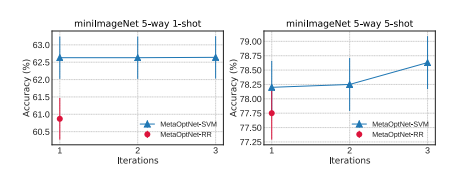
\includegraphics[width=.6\linewidth]{figure/f3.png}
    \caption{使用不同的元训练样本数量,在miniImageNet元测试集上的测试准确率(\%)。}
    \label{fig:3}
\end{figure}

\vspace*{6pt}

\endgroup
\begingroup
\let\clearpage\relax

\chapter{结论与展望}

\section{结论}
本文实现了一种基于凸基学习器的元学习方法,用于少样本学习。
通过利用对偶形式和KKT条件,可以实现计算和内存高效的元学习,
特别适用于少样本学习问题。与最近邻分类器相比,
线性分类器在适度增加计算成本的情况下提供更好的泛化能力(如表\ref{table:3}所示)。
本文的实验表明,正则化线性模型可以在减少过拟合的同时实现显著更高的嵌入维度。
\section{未来展望}
本文提出的将正则化线性分类器作为基础学习器在泛化性上具有较强优势。未来的研究方向是探索其他凸基学习器作为基础学习器在元学习模型中的应用,例如核SVM等,探究更进一步优化时间复杂度的方法。
这将允许更多的训练数据可用于任务,从而逐步增加模型容量的能力。
\endgroup